\chapter{Object Selection}
\label{chap:Objects}

Objects described in \autoref{chap:Reco}, referred to as ``candidates'', are further selected with more stringent requirements with the goal of suppressing the contributions from background processes while maintaining a high signal acceptance. In particular, prompt electron and muon candidates are identified through a custom-trained \ac{BDT} classifier, which is discussed in \autoref{sec:Leptons}. Two jet identification algorithms are deployed to select jet candidates originating from hard collisions, which is discussed in  \autoref{sec:Jets}. Furthermore, jet candidates that originate from b quarks are identified with a \ac{NN} based algorithm, which is discussed in \autoref{sec:Btag}. 
%%%%%%%%%%%%%%%%%%%%%%%%%%%%%%%%%%%%%%%%%%%%%%%%%%%%%%%%%%%%%
%%%%%%%%%%%%%%%%%%%%%%%%%%%%%%%%%%%%%%%%%%%%%%%%%%%%%%%%%%%%%
\section{Lepton Selection}
\label{sec:Leptons}

The target final states of this analysis feature exactly three leptons that originate either from decays of electroweak bosons or from the \ac{CLFV} interaction, which in this analysis is a contact interaction that involves four fermions. These leptons, referred to as \emph{prompt} leptons, typically appear to be isolated and not far away from the \ac{PV}. In contrast, \emph{nonprompt} leptons are leptons that originate from decays of hadrons, or from photon conversions, or misidentified leptons. They often travel a noticeable distance away from the \ac{PV} and appear to be less isolated due to nearby activities. Due to the high multiplicity of leptons in our selection, backgrounds with at least one \emph{nonprompt} lepton outnumber any other \ac{SM} processes that produce three or more \emph{prompt} leptons. It is therefore crucial to exploit the differences between \emph{nonprompt} and \emph{prompt} leptons and bring the \emph{nonprompt} background under control. 
%%%%%%%%%%%%%%%%%%%%%%%%%%%%%%%%%%%%%%%%%%%%%%%%%%%%%%%%%%%%%
\subsection{TOP LeptonMVA}
\label{sec:TOPMVA}

The \TOP is an offline lepton identification algorithm that is originally developed for tZq analyses \cite{CMS:2018sgc,CMS:2021ugv}. It is based on Gradient \ac{BDT} implemented using the TMVA package~\cite{TMVA:2007ngy}. A total of 13 features are used as input to the \ac{BDT}. They can be categorised into four groups: (i) positions and momenta of the lepton candidates, (ii) isolation variables, (iii) variables associated to the closest jet, and (iv) a quality variable that is specific to electron or muon candidate. The version of \TOP used by this analysis is the same as \cite{CMS:2021ugv}, where a detailed description of all input features can be found.

\emph{Prompt} leptons from $\ttbar$W, $\ttbar$Z, and tZq samples are used as signals in the \ac{BDT} training while \emph{nonprompt} leptons from $\ttbar$ samples are used as backgrounds. The trained \ac{BDT} outputs a single score for each lepton candidate ranging from -1 to 1 with -1 (1) being the most background- (signal-) like. the tight working point with a threshold of ($>$) 0.9 is chosen as the selection criteria for both electron candidates and muon candidates, which corresponds to a signal(background) efficiency of 90\%(1\%). The strategy is to trade a small percentage (<10\%) of signal efficiency for several factors of background rejection. 
%%%%%%%%%%%%%%%%%%%%%%%%%%%%%%%%%%%%%%%%%%%%%%%%%%%%%%%%%%%%%
\subsection{Full Selection}
In addition to the \TOP requirement, a set of common selection criteria are applied to both electron and muon candidates. The minimum $\pt$ requirement is 38GeV, 20 GeV, and 20 GeV for the leading, sub-leading, and trailing lepton in $\pt$, respectively. This requirement is driven by the $\pt$ thresholds of the \ac{HLT} triggers to avoid inefficiency at turn-on. Electron and muon candidates are required to be in the pseudorapidity range $|\eta|<$2.4, which corresponds to the acceptance of \ac{CMS} tracker and muon system  in 2016-2018. The transverse (longitudinal) impact parameters with respect to the \ac{PV}, denoted as $d_{\textsf{xy}}$ ($d_{\textsf{z}}$), is required to be in the range $|d_{\textsf{xy}}|~<$ 0.05 cm ($|d_{\textsf{z}}|~<$ 0.05 cm). The significance of the 3-dimensional impact parameter, denoted as SIP$_3$, is defined as the 3-dimensional impact parameter divided by its uncertainty. It is required that SIP$_3$ $<$ 8. The three cuts on impact parameters are added due to the difference in distributions of these parameters between \emph{prompt} and \emph{nonprompt} leptons. Also, they are part of the pre-selection requirement in the \ac{BDT} training.

Furthermore, all lepton candidates are required to be isolated. This is achieved by first defining a cone with a distance parameter of $\mathrm{\Delta}R$ around each lepton candidate, where $\mathrm{\Delta}R=\sqrt{\mathrm{\Delta}\eta^2+\mathrm{\Delta}\phi^2}$. Only particles within $\mathrm{\Delta}R<R_{\textsf{max}}$ can contribute to the isolation variable, where $R_{\textsf{max}}$ is referred to as the size of the cone. Secondly, a \ac{PF} based isolation variable is defined as,

\begin{equation}
I^{\textsf{rel}}_{\textsf{mini}} = \frac{1}{p_{\textsf{T}}^{\ell}} \{\sum_{\textsf{charged}}\pt+\max(0,\sum_{\textsf{neutral}}\pt-\rho \mathcal{A}[\frac{\mathrm{\Delta}R}{0.3}]^2)\},
\end{equation}

where $p_{\textsf{T}}^{\ell}$ is the $\pt$ of the lepton candidate, the first term inside the curly braces is the scalar sum of all charged particles associated with the \ac{PV} while the second term evaluates the contribution from neutral particles. This is done by first scalar-summing over $\pt$ of all neutral particles associated to the \ac{PV}. A correction term, known as effective area correction~\cite{Cacciari:2007fd}, is then subtracted. This term is used to mitigate the impact of \ac{PU} interactions. The size of the cone scales with $p_{\textsf{T}}^{\ell}$ as,  

\begin{equation}
R_{\textsf{max}} = \max (0.05, \min(0.2, \frac{10\GeV}{p_{\textsf{T}}^{\ell}})).
\end{equation}.

This type of isolation variable is known as ``mini'' isolation, which maximises the signal efficiency at $p_{\textsf{T}}^{\ell}$ by reducing the cone size. It is required that lepton candidates to have $I^{\textsf{rel}}_{\textsf{mini}}<$ 0.12.

For electron specifically, candidates are required to have a GSF track with one of less missing inner hit. Electron candidates reconstructed in the transition region between ECAL barrel and endcap (i.e. 1.44 $<~|\eta_{\textsf{SC}}|~<$ 1.57) are removed from consideration. For muon specifically, candidates are required to be \ac{PF} muons and pass the medium working point discussed in \autoref{sec:Muon}.

Lepton candidates that pass all requirements stated above are referred to as ``\emph{tight}'' leptons. Leptons selected with a separate set of criteria, known as ``\emph{loose}'', is used in estimating the \emph{nonprompt} background, which is discussed in \autoref{chap:Nonprompt}. Unless explicitly stated, all lepton objects presented in this search are \emph{tight} leptons.

The energy of electron candidates are calibrated through. The moment scale of muon candidates are calibrated for muon candidates with $\pt~<$ 200 GeV. Scale factors are applied to \emph{tight} leptons to correct for the differences in reconstruction, isolation, and identification between data and \ac{MC}. These scale factors are obtained using dilepton events in Z resonance window.
%%%%%%%%%%%%%%%%%%%%%%%%%%%%%%%%%%%%%%%%%%%%%%%%%%%%%%%%%%%%%
%%%%%%%%%%%%%%%%%%%%%%%%%%%%%%%%%%%%%%%%%%%%%%%%%%%%%%%%%%%%%
\section{Jet Selection}
\label{sec:Jets}

Jet candidates are reconstructed from \ac{PF} candidates using the anti-$k_{\textsf{T}}$ algorithm described in \autoref{sec:Jets} with a cone size of 0.4. Charged hadrons that are not associated to the \ac{PV} are removed. Jet candidates are required to have a minimum $\pt$ of 30 GeV and in in the pseudorapidity range $|\eta|<$2.4, where b-tagging are still effective. It is further required that all jet candidates to be isolated from \emph{tight} leptons. A cone of the size 0.4 around each jet candidate is defined and candidates will be removed if any \emph{tight} leptons are found within such a cone. This procedure is implemented to remove the overlap between leptons and jets. 

The two primary sources of background are (i) detector noise, and (ii) jets from \ac{PU} interactions. To suppress detector noise, a set of cut-based selections are applied to jet candidates. This algorithm utilizes information from \ac{PF} candidates, including: (i) fraction of charged (neutral) hadrons energy, (ii) fraction of charged (neutral) EM energy, (iii) fraction of muon energy, and (iv) object multiplicity. The ``tightLepVeto'' working point is chosen to select jet candidates, which corresponds to 98-99\% signal efficiency.

The second algorithm is designed to reject jet candidates that originate from \ac{PU} interactions. This algorithm is based on a \ac{BDT} that utilizes: (i) the trajectories of tracks associated to the jets, (ii) the topology of the jet shape, and (iii) object multiplicity. The \emph{loose} working point is chosen to select jet candidates with $\pt~<$ 50 GeV, which corresponds to 99\% signal efficiency. Applying this algorithm to jet candidates with $\pt~>$ 50 GeV is both ineffective and unnecessary as \ac{PU} jets mostly reside in low $\pt$ spectrum. The overall effect of this algorithm on this analysis is small as \ac{PU} jets constitute only a small fraction of all jet candidates in the phase space of this analysis. 

As discussed in \autoref{sec:Jet}, the energy scale for all jet candidates (data and \ac{MC}) are calibrated. One extra correction is applied to simulated jets to recreate the jet energy resolution as measured in data. 
%%%%%%%%%%%%%%%%%%%%%%%%%%%%%%%%%%%%%%%%%%%%%%%%%%%%%%%%%%%%%
%%%%%%%%%%%%%%%%%%%%%%%%%%%%%%%%%%%%%%%%%%%%%%%%%%%%%%%%%%%%%
\section{Identification of b jets}
\label{sec:Btag}

The \DeepJ algorithm~\cite{Bols:2020bkb} is used to identify jets that originate from b quark. The core strategy of this algorithm is to minimise information. This is achieved by removing entirely the selection of jet constituents, which limits the number of jet constituents considered.  Additionally, an effort is made to use as many low-level features as possible, which further further deepens the feature space. Approximately a total of 650 input features are used,  which can be categorized into four groups: (i) global variables, (ii) charged PF candidate features, (iii) neutral PF candidate features, (iv) and \ac{SV} features associated with the jet. 

The \DeepJ algorithm outputs a score ranging between 0 and 1, with 0 (1) being the most background- (signal-) like. The medium working point is chosen to tag b jet candidate, which corresponds to 90\% signal efficiency. The shape of the \DeepJ output distribution is corrected for the differences between data and \ac{MC} in signal and background efficiencies. The per-event correction weight $ \omega$ is defined as,
 
 \begin{equation}
 \omega = \prod_{i}^{N_{\textsf{jets}}} \textsf{SF}(p_{T_{i}},\eta_i, F_i, D_i),
 \end{equation}
 
where \textsf{SF} is the ratio of efficiency in data to efficiency to \ac{MC} parameterized as a function of $\pt$, $\eta$, (MC truth) flavor F, as well as \DeepJ output $D$ of each jet in the event. $\omega$ is applied to all \ac{MC} samples, and additional scale factors are also applied to remove the normlization effect of $\omega$. These scale factors are measured using \ac{MC} in e$\upmu\ell$ channel described in \autoref{chap:Selection}. The effect of these scale factors are shown in Figure~\ref{fig:BtagSF}.
 
 \begin{figure}[tbh!]
 \begin{center}
 \begin{tabular}{c}
 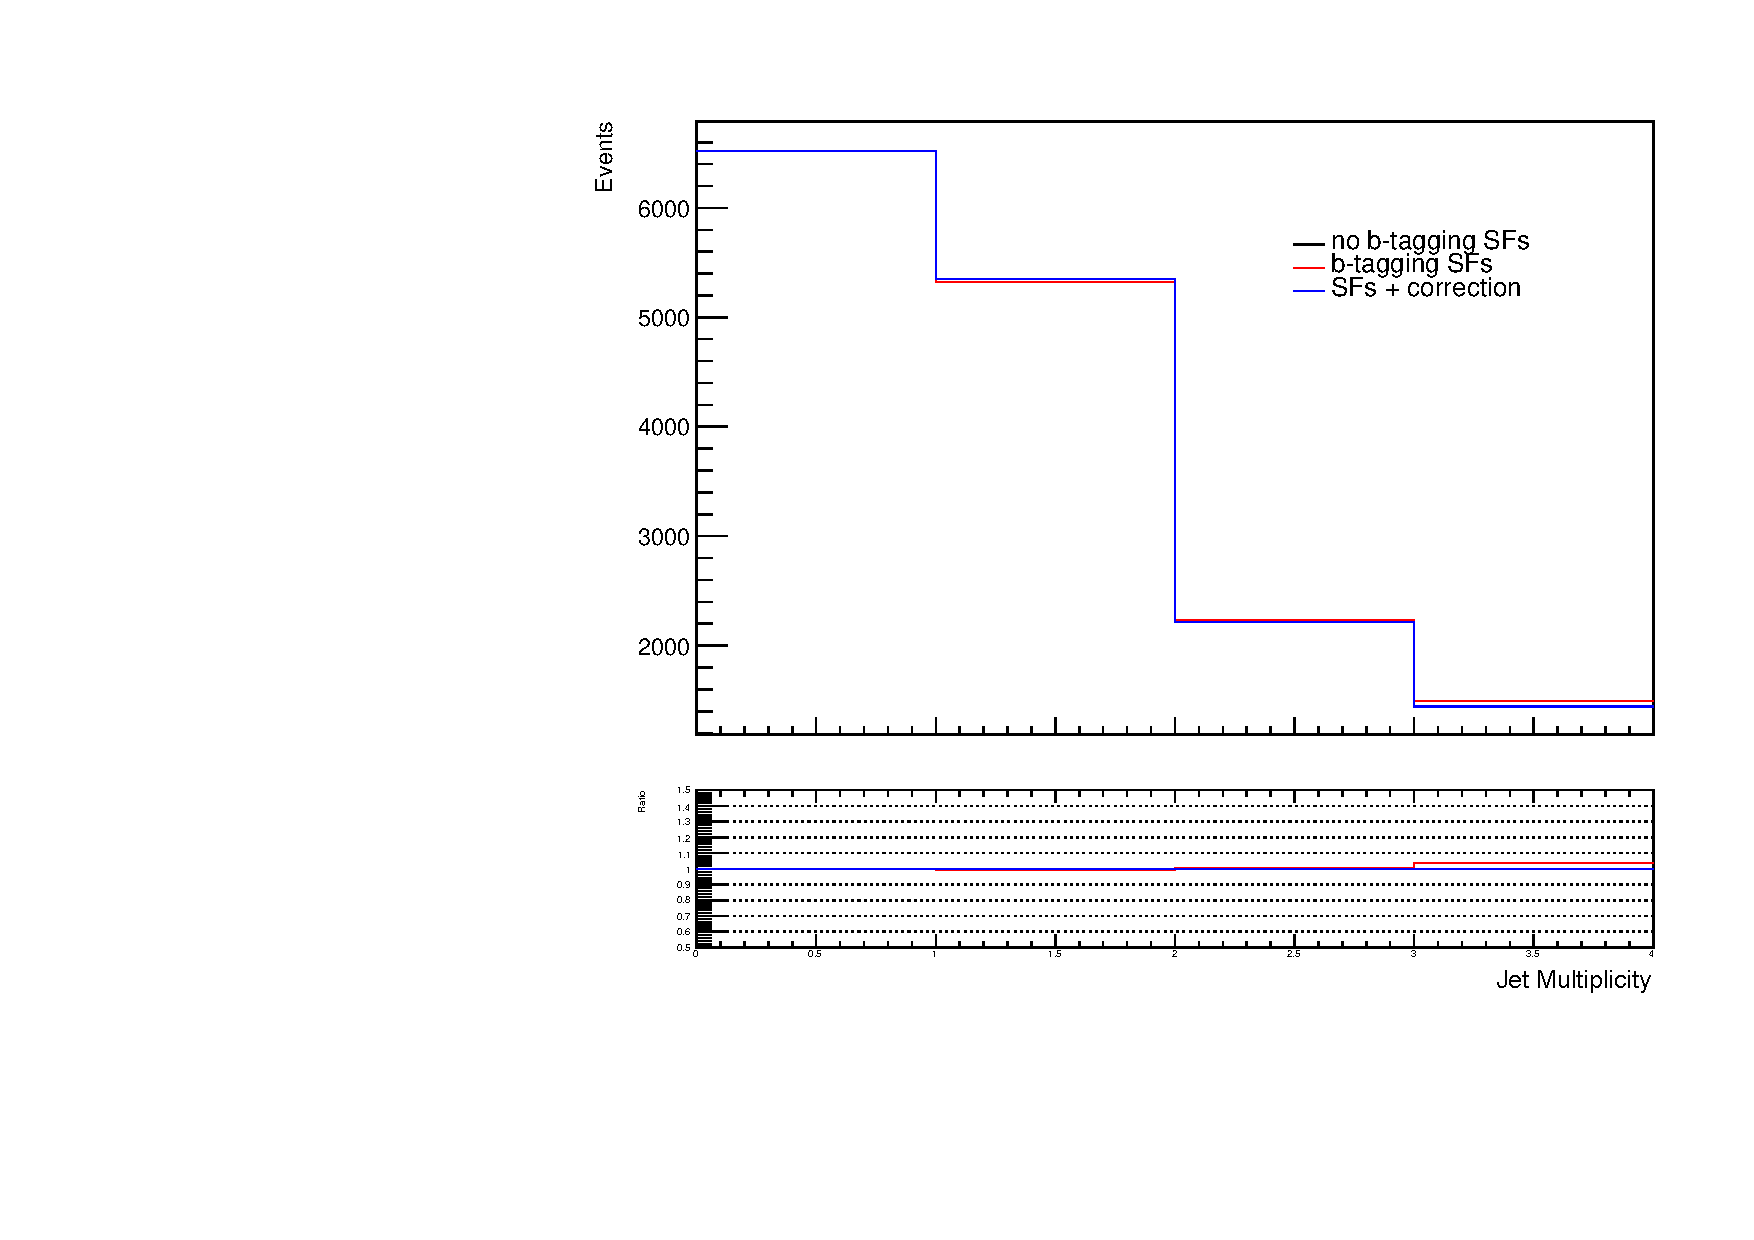
\includegraphics[width=0.75\textwidth]{figures/Part3/Objects/njet_Btag}\\
 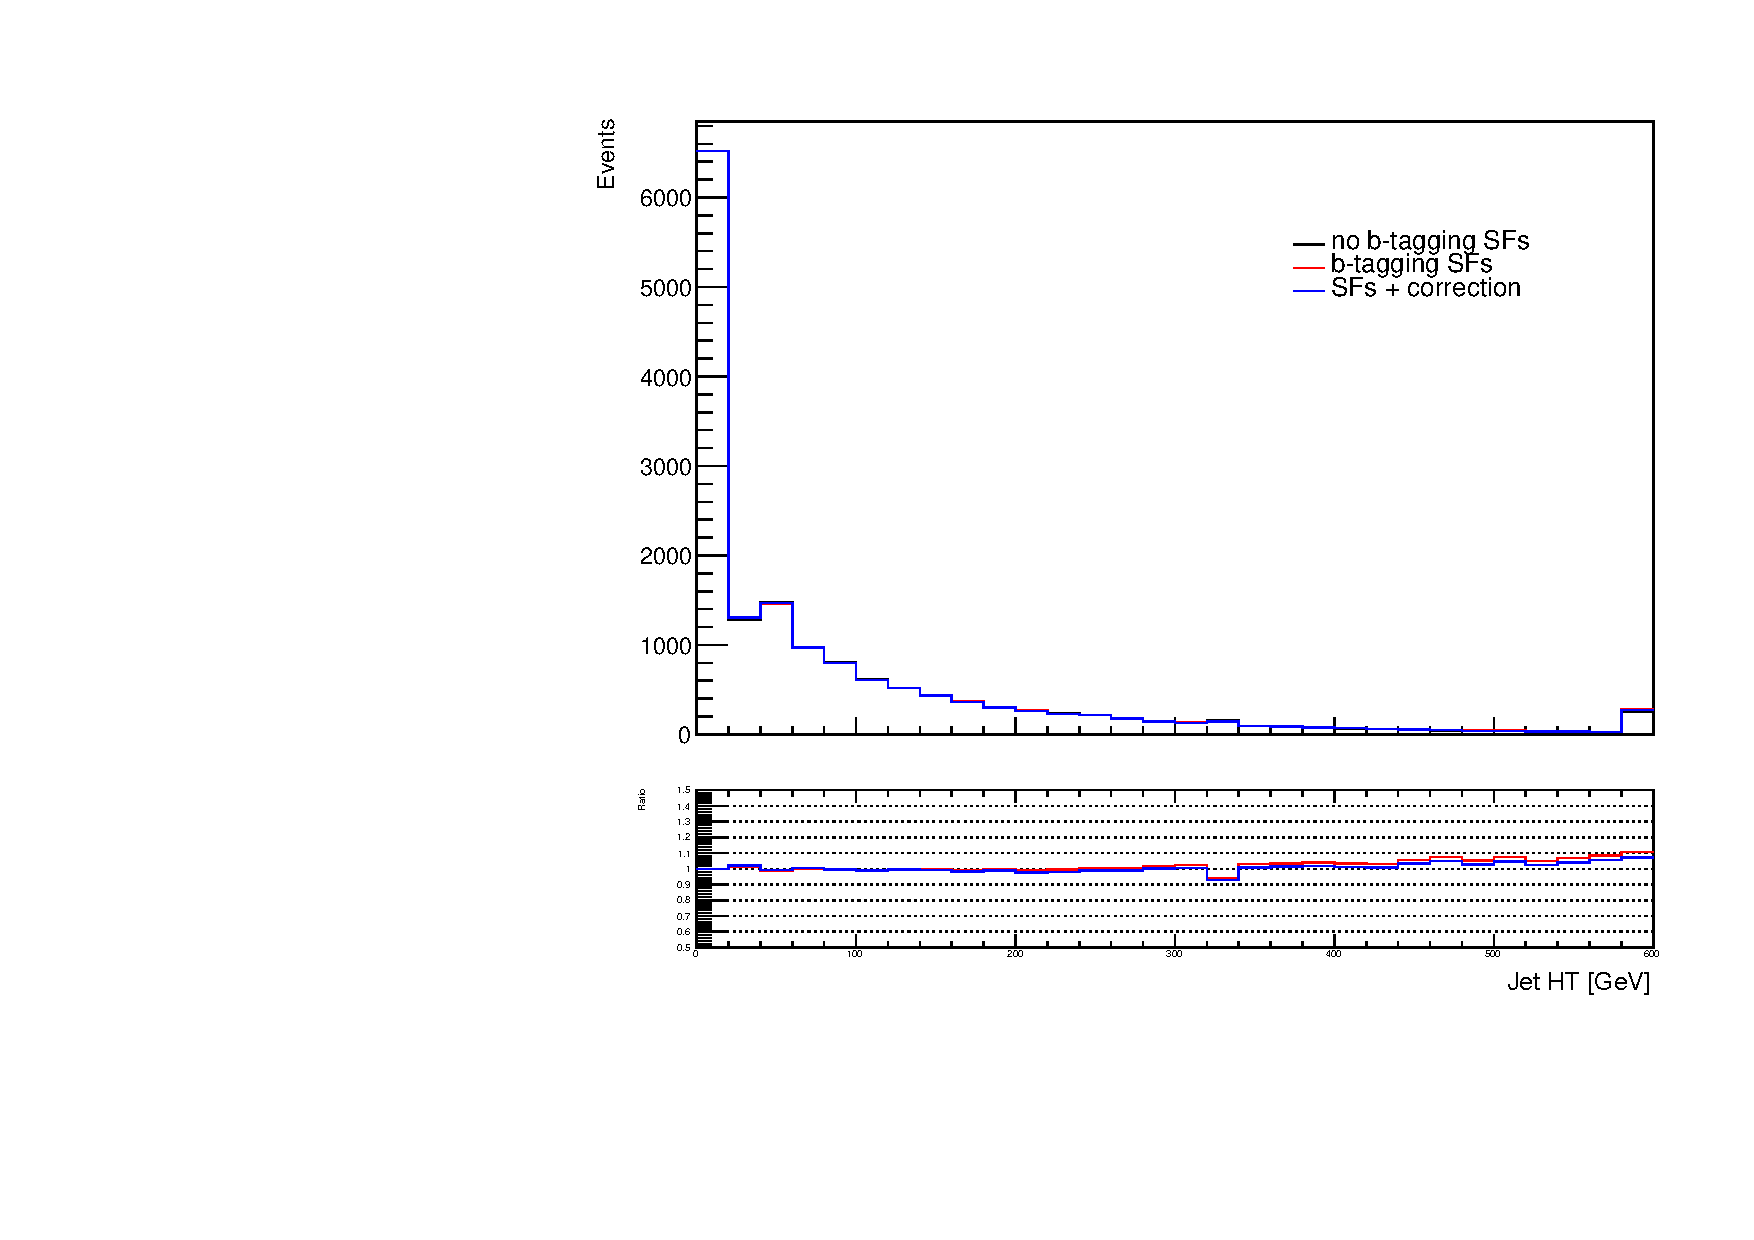
\includegraphics[width=0.75\textwidth]{figures/Part3/Objects/Ht_Btag} \\
 \end{tabular}
 \caption{Simulated events in $e\mu l$ channel (run-II). Top: jet multiplicity. Bottom: $H_T$ of jets.}
 \label{fig:BtagSF}
 \end{center}
\end{figure}